
\begin{figure*}[!bt]
	\begin{minipage}{4cm}
		\centering
		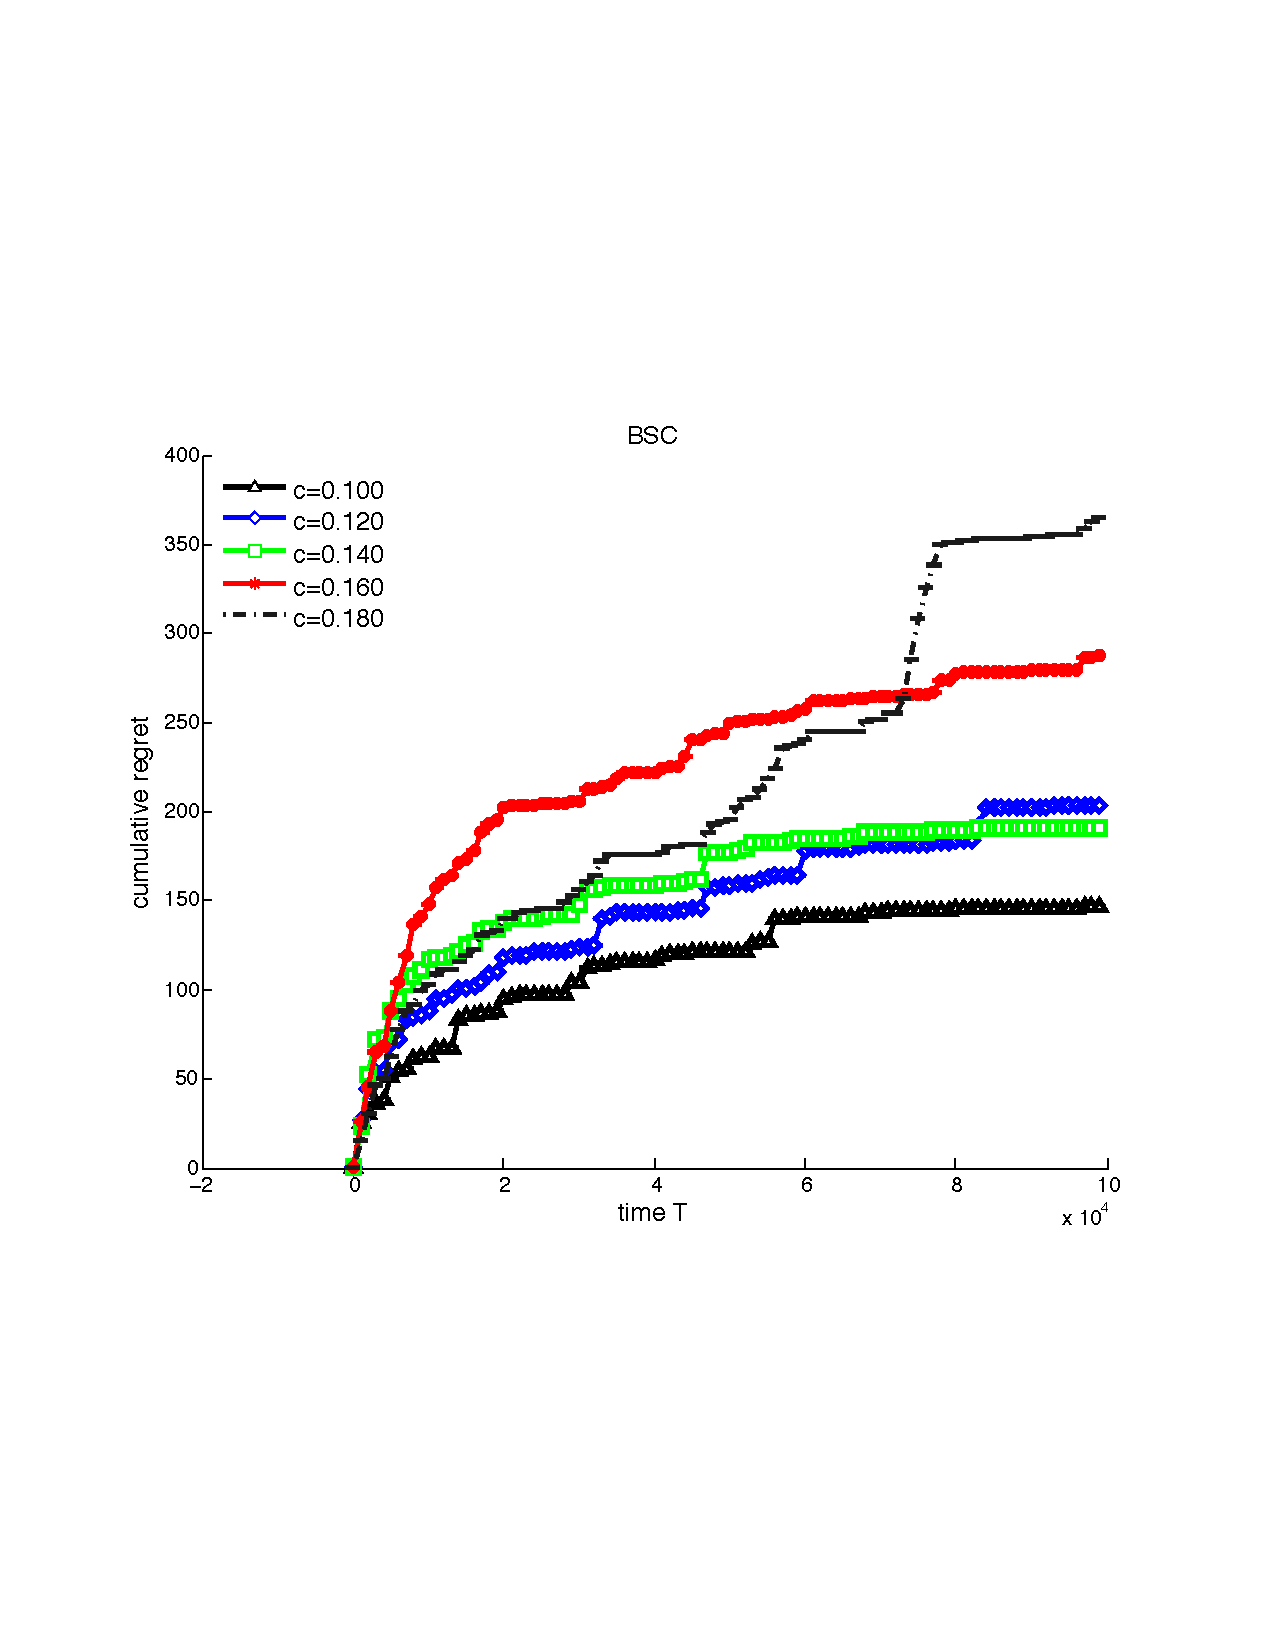
\includegraphics[scale=0.21]{../Simulations/Figures/BSC_SD}
		\label{fig:BSC_SD}
		\vspace{-.2cm}
		\caption{BSC data satisfying SD}
	\end{minipage}
	\begin{minipage}{4cm}
		\centering
		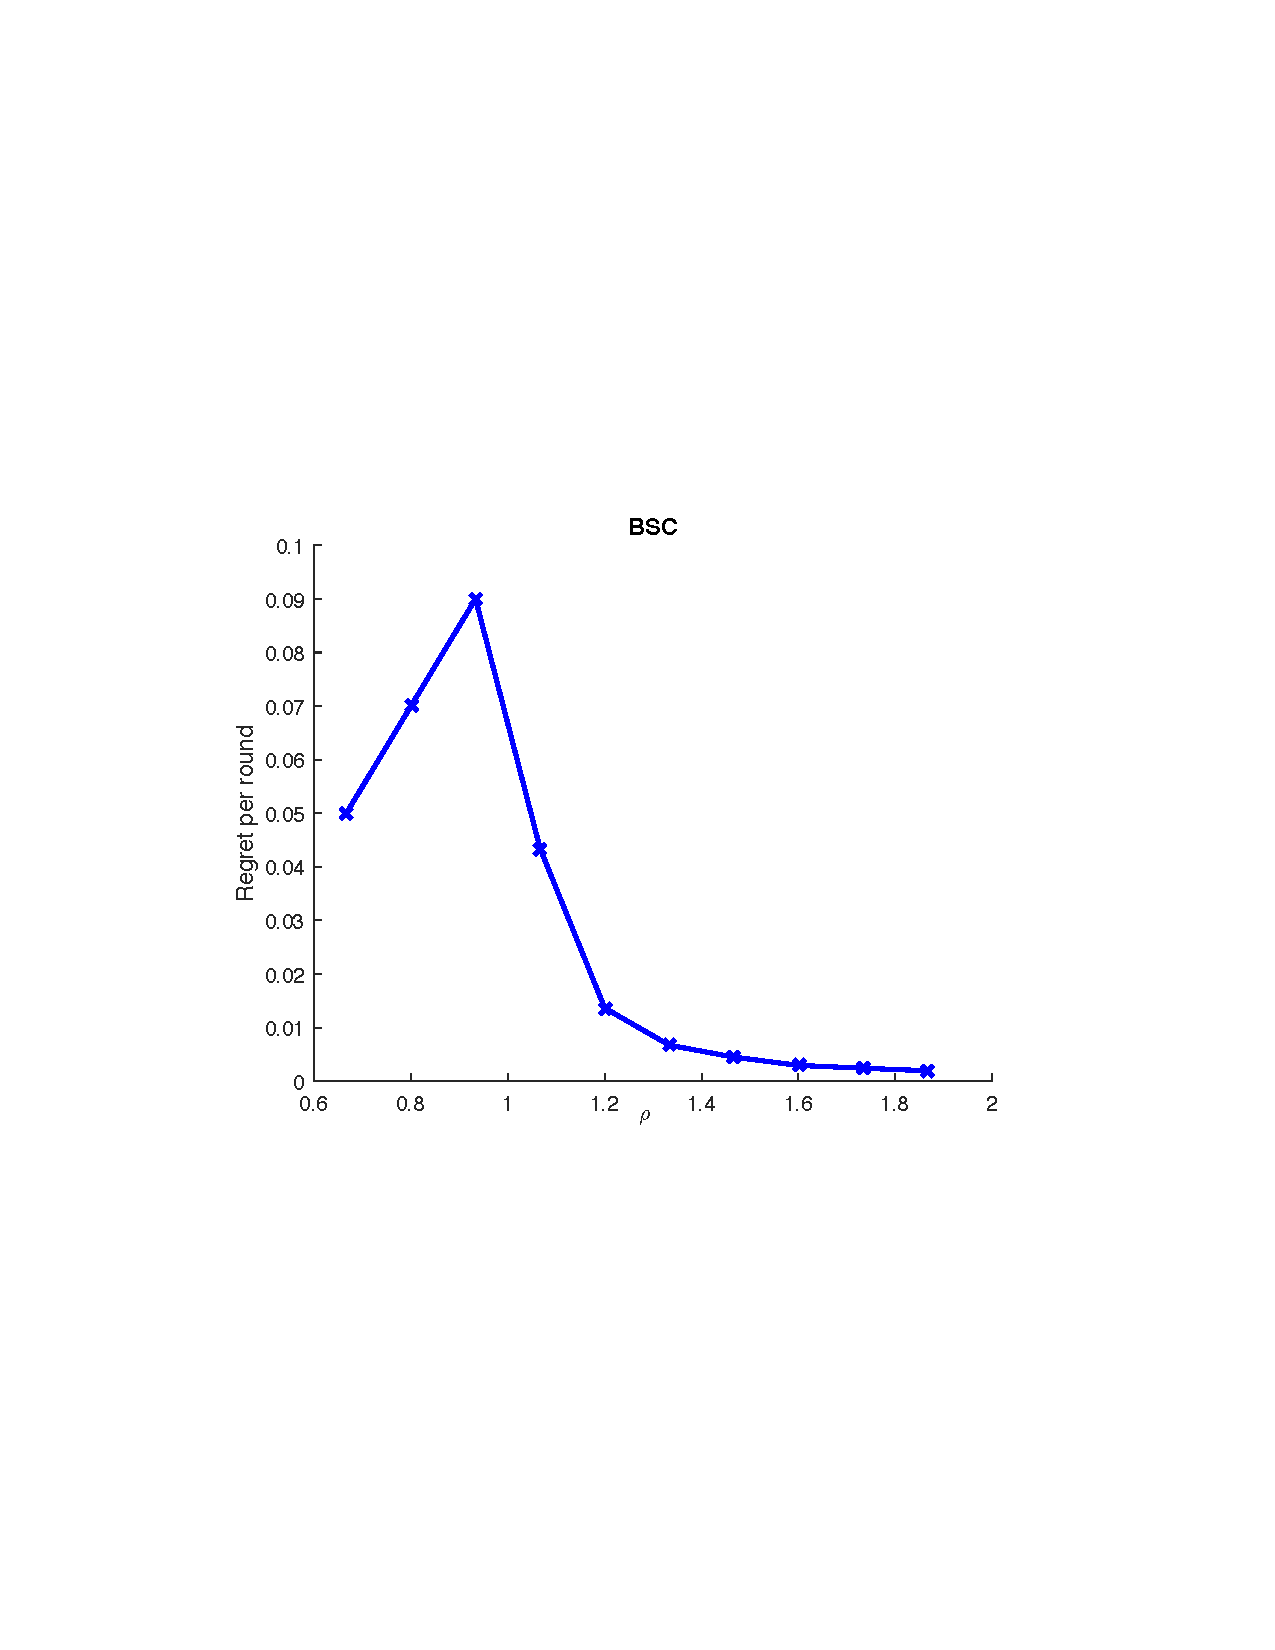
\includegraphics[scale=0.3]{../Simulations/Figures/BSC_WD1}
		\label{fig:BSC_WD}
		\vspace{-1cm}
		\caption{BSC data}
	\end{minipage}
	\begin{minipage}{4cm}
		\centering
		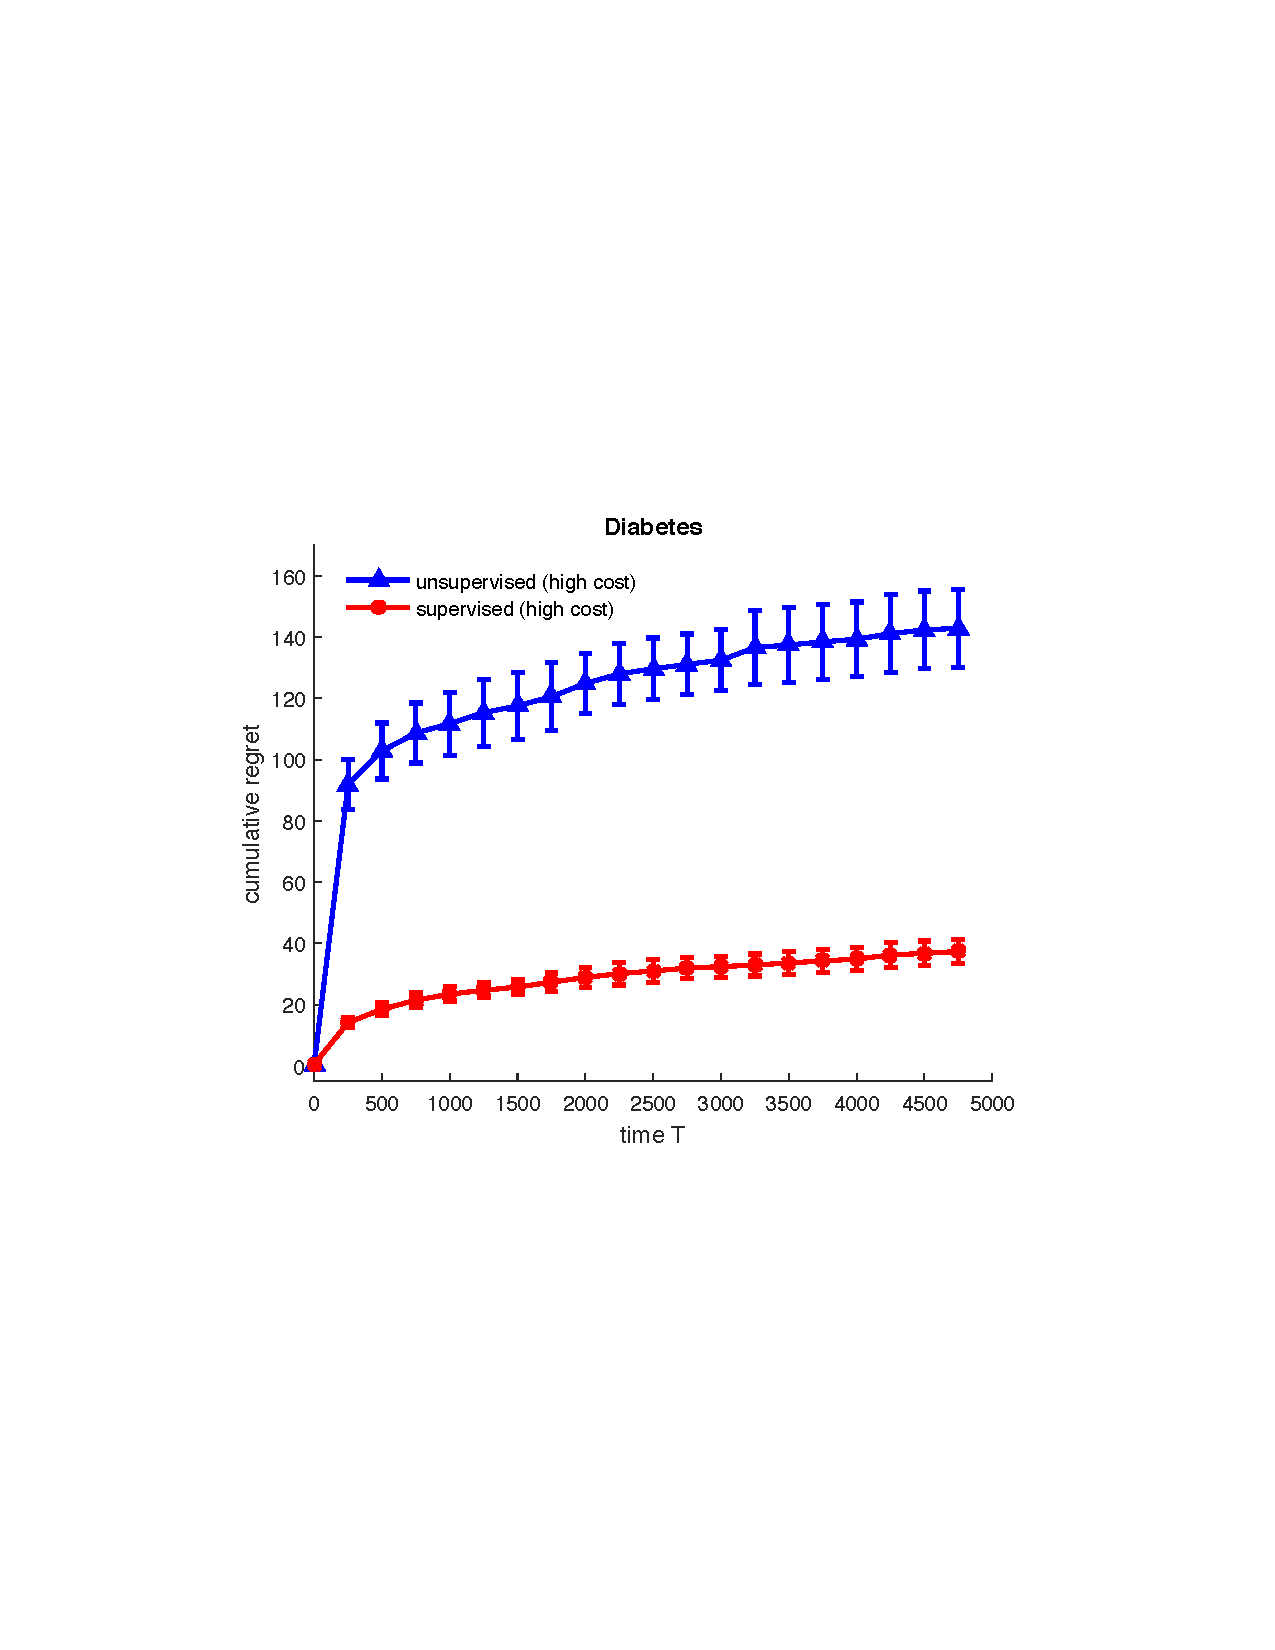
\includegraphics[scale=0.3]{../Simulations/Figures/Diabetes_WD1}
		\label{fig:Diabetes}
		\vspace{-1cm}
		\caption{Diabetes dataset}
	\end{minipage}
	\begin{minipage}{4cm}
		\centering
		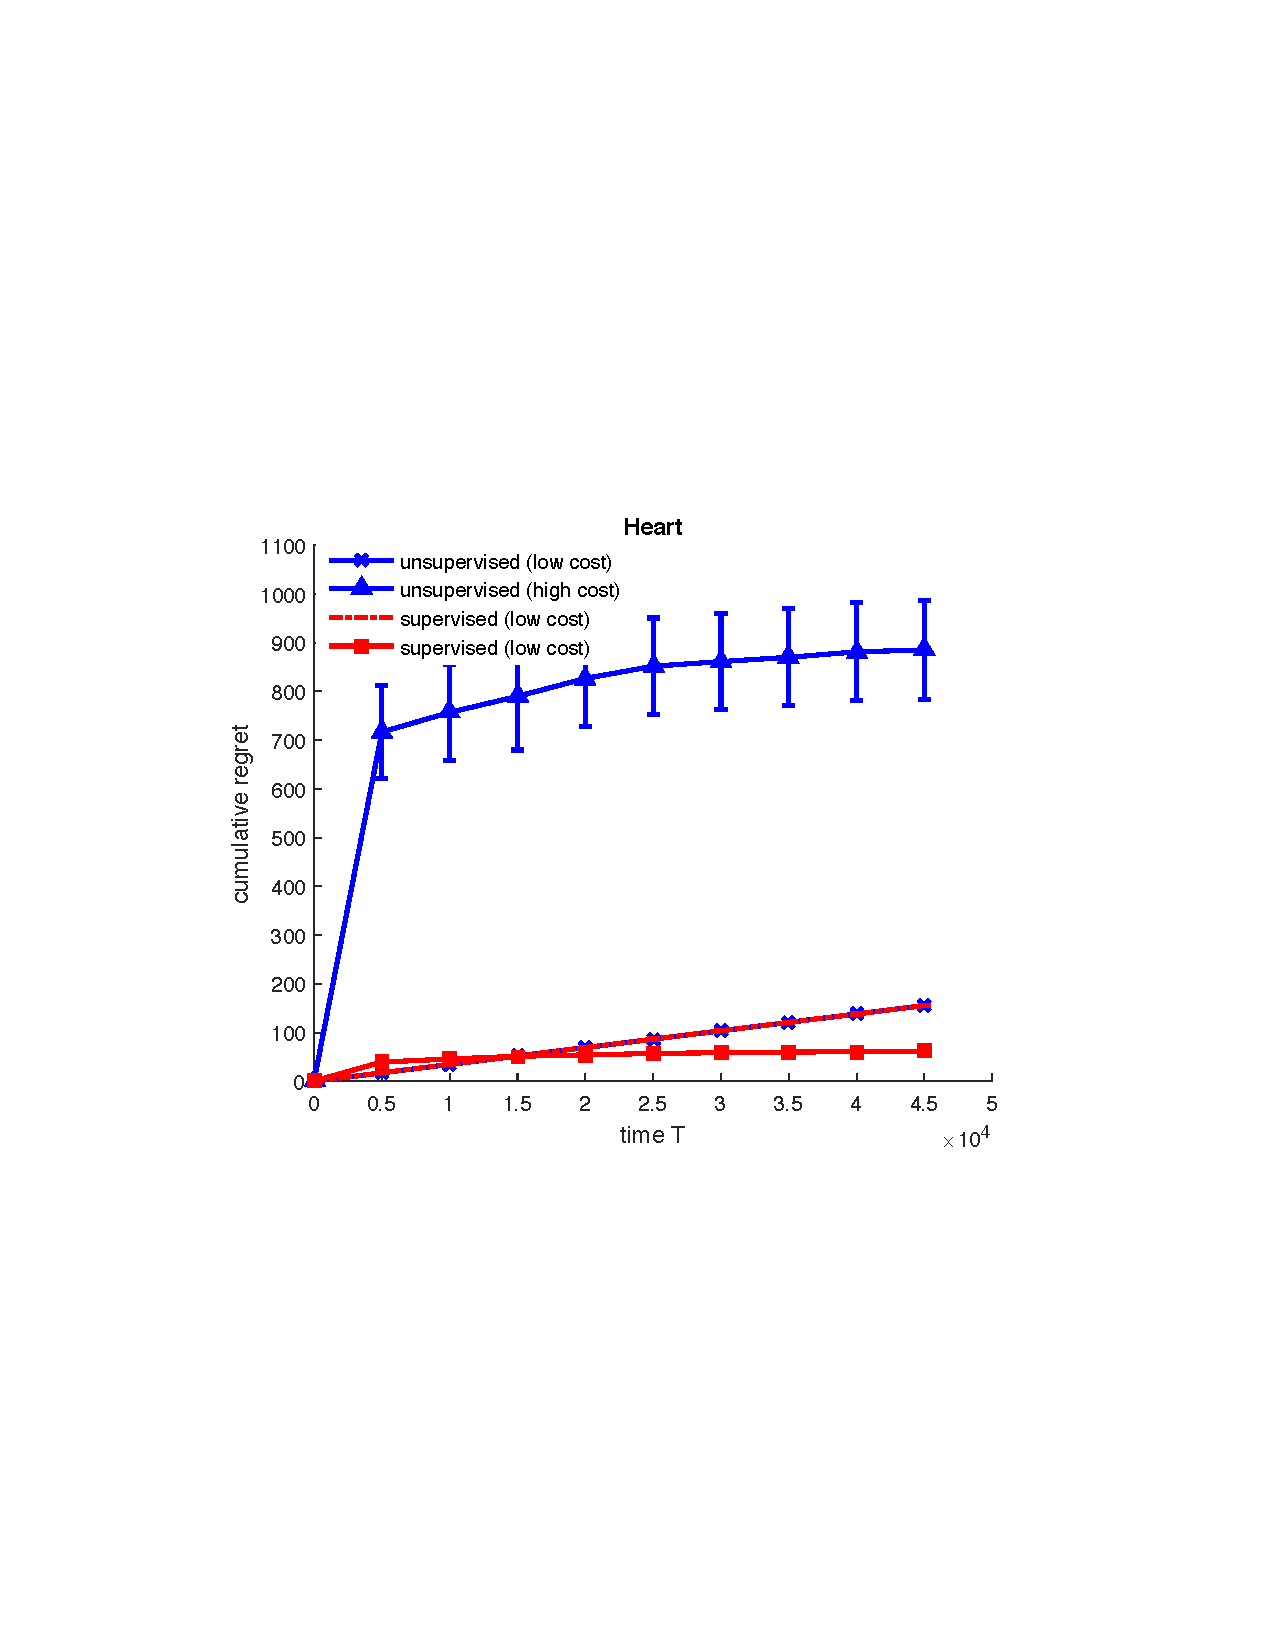
\includegraphics[scale=0.3]{../Simulations/Figures/Heart_WD1}
		\label{fig:Heart}
		\vspace{-1cm}
		\caption{Heart dataset}
	\end{minipage}
	\vspace{.2cm}

\noindent
In Fig. \ref{fig:BSC_SD}, BSC data is generated that satisfies SD property and Algorithm \ref{alg:asym} is applied. In  Fig. \ref{fig:BSC_WD}, Algorithm \ref{alg:UCB} is applied on BSC data. In Fig. \ref{fig:Diabetes} Algorithm \ref{alg:UCB} and the standard UCB algorithm are applied on the Diabetes dataset. In Fig. \ref{fig:Heart}, Algorithm \ref{algo:UCB} and standard UCB algorithm are applied on the heart dataset. 
\end{figure*}

In this section we evaluate performance of Algorithms \ref{alg:asym} and \ref{alg:UCB} on synthetic and real datasets. For synthetic example, we consider data transmission over a binary symmetric channel, and for real world examples, we use diabetes (PIMA indiana) and heart disease (Clevland) from UCI dataset. In both datasets attributes/features are associated with costs, where features related to physical observations are cheap and that obtained from medical tests are costly. The experiments are setup as follows:

{\bf Synthetic:} we consider data transmission over three binary symmetric channels (BSCs). Channel $i=1,2,3$ flips input bit with probability $p_i$ where $p_1\geq p_2\geq p_3$. Transmission over channel $1$ is free and that over channel $2$ and $3$ costs price of $ c_2$ and $c_3\in (0,1] $ units per bit, respectively. Input bits are generated with probability $0.7$ and we set $p_1=.4, p_2=.1$ and $p_3=.05$.

{\bf Datatsets:} we obtain a sensor acquisition setup from the datasets as follows: Three svm classifiers (linear, $C=.01$) are trained for each dataset, first one using only cheap features, second one  using cheap features plus few additional features and the third one using all features. These classifiers form sensors of a three stage SAP where classifier trained with cheap features is the first stage and that trained with all the features forms the last stage. Cost of each stage is the sum of cost of features used to train that stage multiplied by a scaling factor $\lambda$ (trade-off parameter between prediction accuracy and costs). Specific details for each dataset is given below.  

{\bf PIMA indians diabetes} dataset consists of $768$ instances and has $8$ attributes. The labels identify if the instances are diabetic or not. First sensor of SAP is trained with $4$ cheap attributes and costs \$$4$ (times-pregency, pedigree, diastolic-pb, triceps ). Second sensor is trained from $7$ attributes that includes age, mass-index and insulin in addition to the attributed used for the first sensor and cost total of \$$29$, and the last sesnor is trained with all $8$ attributes that cost \$$46$. We set $C_1= 4\lambda, C_2= 29\lambda$ and $C_3= 46\lambda$.
% $6$ of the attributes obtained from physical observations are cheap, and $2$ attributes (glucose and insulin) require expensive tests. 

{\bf Heart disease} dataset consists of $297$ instance (without missing values) and has $13$ attributes. $5$ class labels $(0,1,2,3,4)$ are mapped to binary values by taking value $0$ as `absence' of disease and values $(1,2,3,4)$ as `presence' of disease. First senor of SAP is trained with first $7$ attributes which cost  \$$32$ in total, second sensor is trained with first $11$ attributes that cost \$$1$ each and the third sensor is trained with all the attributes  cost total of \$$568$. We set $C_1= 32\lambda, C_2= 397\lambda$ and $C_3= 601\lambda$.
	\begin{figure}[!h]
		\small
		\begin{tabular}[c]{c|c|c|c|c|c|c } 
			\label{tab:ErrorTable}
			%	\caption{cap:Error statistics}
			dataset & $\gamma_1$ & $\gamma_2$ & $\gamma_3$ &$\delta_{12}$ & $\delta_{13}$ & $\delta_{23}$ \\ \hline 
			BSC & .3 & .1 & .05 & .07 & .035 & .045\\  \hline
			diabetic & $0.345 $ & $ 0.324$ & 0.246 & $ 0.116 $ & 0.089 &0.058\\  \hline
			heart & $0.292$ & $0.27$ & 0.146 & $0.124$ & 0.067 & 0.079\\  \hline
		\end{tabular}
		\caption{Error statistics for real and synthetic datasets. $\delta_{ij}:=\P\{Y^i=Y, Y_j\neq Y\}$.}
	\end{figure}

Various error probabilities for synthetic and datasets are listed in Table (\ref{tab:ErrorTable}).  
The probabilities for the datasets are computed on $40 \%$ hold out data. To run the online algorithm, an instance is randomly selected from the dataset (with replacement) in each round and is input to the  algorithm. We repeat the experiments $20$ times and average is shown in figures (\ref{fig:BSC_SD}-\ref{fig:Heart}) with $95\%$ confidence bounds. 
Fo the synthetic experiments we set $c_1=0$ and $c_2+c_3=0.4$ while varying $c_2$ between $[0.1 0.29]$. The optimal action in this setup is $2$. In Figure \ref{fig:BSC_SD} we applied Algorithm \ref{alg:asym} on BSC data that satisfies SD property. As seen, the algorithm learns the optimal arm for all values of $c_2$. In Figure \ref{fig:BSC_WD} 
we applied Algorithm \ref{alg:UCB} on BSC data, where The $x$-axis in the figure is the ratio
\[R= \frac{0.4 - c_2}{\Pr\{Y^2 \neq Y^3\}}\]
and $y$-axis is the regret per round. As shown,  regret per round is small when $R>1$, whereas it is high for for $R<1$. This observation follows by applying definition of (\ref{dfn:WDP})- when $R>1$, the setup satisfies the WD property and the algorithm identifies the optimal action, whereas when $R<1$ the setup violates the WD property and the algorithm cannot identify the optimal arm. This validates the learnability under the WD property. 

In figure \ref{fig:Diabetes}, we apply Algorithm $2$ and standard UCB algorithm on the Diabetes dataset. In applying the standard using algorithm, we use the true label in each round to get the loss for the action played. The regret plots corresponding to the Algorithm $2$ are labeled as unsupervised and that corresponding to standard UCB as supervised in the figure. We consider two values for trade-off factor, $\lambda=0.001$ and $\lambda=0.015$. In the first case, accuracy is given higher weight and action $3$ is optimal, in the second cost factor becomes dominant and action $1$ is optimal. When action $3$ is optimal, the performance of both the supervised and unsupervised methods are almost identical. When action $1$ is optimal. As expected, the performance of unsupervised method is better than the supervised method, but unsupervised method learns the optimal arms almost after the same number of rounds as the supervised method though it incurs high regret in the initial rounds.
  

In figure \ref{fig:Heart} we again apply Algorithm $2$ on the standard UCB algorithm on the heart dataset. We set $\lambda=0.05$ for which action $1$ is optimal. The two corresponding plots are labeled as unsupervised and supervised in the figure. We also plot the regret obtained when noisy labels are input to the 
the standard UCB algorithm instead of the true labels. This plot is labeled as supervised (noisy) in the figure which is obtained when each label is flipped by probability $0.2$. As seen, the regret performance of the supervised method deteriorates as label gets noisier. 


